\documentclass[../main]{subfiles}

\begin{document}

\section{最大離陸重量$W_{TO}$, 空虚重量$W_{E}$, 燃料重量$W_F$の見積もり }
  $W_{TO}$は、定義式
  \begin{equation}
    W_{OE} = W_{E} + W_{tfo} + W_{crew} + W_{OP}
    \label{eq:w_oe1}
  \end{equation}
  定義式から導出される式
  \begin{equation}
    W_{OE} = W_{TO} - (1-M_{ff})W_{TO} - W_{Fres} - W_{PL}
    \label{eq:w_oe2}
  \end{equation}
  統計関係式
  \begin{align}
    \log{10} W_{TO} = A' + B'\log{10}W_{OE} \label{log10} \\
    \text{ただし,} \ A'=0.4736 \  B'=0.9656 \label{eq:ab}
  \end{align}
  の3式を用いて算出できる.

  \subsection{Mission fuel fraction $M_{ff}$の見積もり}
    $M_{ff}$を見積もる.飛行フェーズを下図のように設定する.
    \begin{figure}[H]
      \begin{center}
        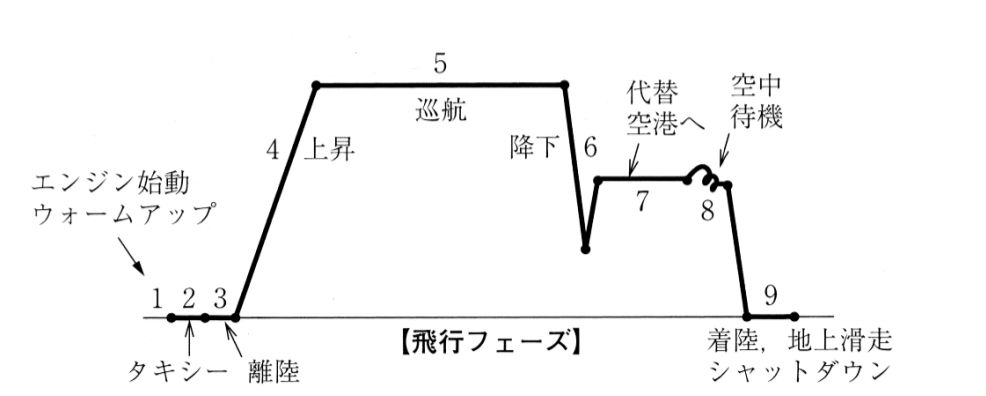
\includegraphics[width=12.0cm]{route.png}
        \caption{飛行フェーズ} %タイトルをつける
        \label{route} %ラベルをつけ図の参照を可能にする
      \end{center}
    \end{figure}
    各フェーズでの重量比を,
    \begin{equation}
      \biggl( \frac{W_1}{W_{TO}},\frac{W_2}{W_1},\frac{W_3}{W_2},\frac{W_4}{W_3},\frac{W_6}{W_5},\frac{W_9}{W_8} \biggr )
      = (0.990,0.990,0.995,0.980,0.990,0.992)
    \end{equation}
    と仮定し,巡行、代替空港への巡行,空中待機のフェーズではブレゲーの式より、
    \begin{align}
      \frac{W_5}{W_4} &= exp \biggl( -\frac{R}{\frac{V}{C_j}\frac{L}{D}} \biggr) \nonumber \\
      \frac{W_7}{W_6} &= exp \biggl( -\frac{R_{alt}}
      {\frac{V_{alt}}{c_{j_{alt}}} \frac{L}{D_{alt}} } \biggr)  \\
      \frac{W_8}{W_7} &= exp \biggl( -\frac{E_{ltr}}
      {\frac{1}{c_{j_{ltr}}} \frac{L}{D_{ltr}} } \biggr) \nonumber
    \end{align}
    である。設計要求から、
    \begin{align}
      R &= 7500 \ [nm] \nonumber \\
      R_{alt} &= 200 \ [nm] \nonumber \\
      V &= M 0.8 \times 574 \ [kt] = 459.2 \ [kt] at 38000 \ [ft] \nonumber \\
      V_{alt} &= 300 \nonumber \\
      \frac{L}{D} &= \frac{L}{D_{alt}} = 20  \\
      c_j = c_{j_{alt}} &= 0.5 \ [(Ib/hr)/Ib] \nonumber \\
      E_{ltr} &= 0.75 \ [hr] \nonumber \\
      \frac{L}{D_{ltr}} &= 23 \nonumber \\
      c_{j_{ltr}} &= 0.4 \nonumber
    \end{align}
    となる。よって,
    \begin{eqnarray}
      \begin{cases}
        \dfrac{W_5}{W_4} = 0.692  & \\[5mm]
        \dfrac{W_7}{W_6} = 0.990  & \\[5mm]
        \dfrac{W_8}{W_7} = 0.987 & \\
      \end{cases}
    \end{eqnarray}
    となり、
    \begin{equation}
      M_{ff} = \frac{W_9}{W_8} \cdot \frac{W_8}{W_7} \cdot \frac{W_7}{W_6} \cdot
      \frac{W_6}{W_5}  \cdot \frac{W_5}{W_4} \cdot \frac{W_4}{W_3}
      \cdot \frac{W_3}{W_2} \cdot \frac{W_2}{W_1} \cdot \frac{W_1}{W_{TO}} = 0.63
    \end{equation}
    となる。
  \subsection{ペイロード重量$W_{PL}$,乗務員重量$W_{crew}$の見積もり}
    乗客の割合をエコノミークラス352名,ビジネスクラス42名,ファーストクラス26名の総員420名とし、
    キャビンアテンダントを15名, パイロット2名とする。計算により,
    \begin{eqnarray}
      \begin{cases}
        & W_{Pl} = 420 \times 175 [Ibs] + 352 \times 44 [Ibs] + (42+26) \times 66 [Ibs] = 93476[Ibs] \\[3mm]
        & W_{crew} = (15 + 2) * (175 + 30) [Ibs] = 3485 [Ibs]
      \end{cases}
    \end{eqnarray}
    となる。

  \subsection{最大離陸重量$W_{TO}$の見積もり}
    最大離陸重量$W_{TO}$から計算される$W_{OE}$と$W_{OE_{tent}}$の差が最小になるような$W_{TO}$
    を決定する。
    代替空港も空中待機も飛行フェーズに含んでいるので、$W_{Fres}=0$としてよく、
    \begin{equation}
      W_F = W_{Fused} = (1-M_{ff})W_{TO} - W_{PL}
    \end{equation}
    となる。また,式(2)より
    \begin{equation}
      W_{OE_{tent}} = W_{TO} - (1-M_{ff})W_{TO} - W_{PL}
    \end{equation}
    よって
    \begin{equation}
      W_{E_{tent}} = W_{OE_{tent}} - W_{crew}
    \end{equation}
    さらに、式(3),(4)より、
    \begin{equation}
      W_{E} = 10 ^ {\frac{log_{10}W_{TO} - A'}{B'}}
    \end{equation}
    $W_{E}$と$W_{E_{tent}}$の差が小さくなるように$W_{TO}$の探索を行った.すると
    \begin{equation}
      W_{TO} = 896000 [Ibs]
    \end{equation}
    の時、
    \begin{eqnarray}
      \begin{cases}
        W_{E_{tent}} = 471952 [Ibs] \\[3mm]
        W_{E} = 471943 [Ibs]
      \end{cases}
    \end{eqnarray}
    となり、収束した.

\end{document}
